\documentclass[a4paper, titlepage, 12pt]{article}
\usepackage[a4paper, margin=2.2cm]{geometry}
\usepackage[utf8]{inputenc}
\usepackage{float, amssymb, amsmath, amsbsy} 
\usepackage{mathdots, mathrsfs, topcapt, multirow}
\usepackage[hidelinks]{hyperref}
\usepackage{graphicx, caption, booktabs}
\usepackage{subfigure}
\usepackage[spanish, es-tabla]{babel}
\usepackage{mathtools, fancyref}
\usepackage{multicol}
\usepackage[x11names,table]{xcolor}
\usepackage{listings}
\usepackage{tikz}
\usepackage{multicol}
\usepackage{amsthm}
\def\proof{\paragraph{Demostraci\'on:\\}}
\def\endproof{\hfill$\blacksquare$}

\newtheorem{thm}{Teorema}[section]


\theoremstyle{definition}%Pone en letra negrita la palabra proposicion,etc 

\newtheorem{de}[thm]{Definición}
\newtheorem{nota}[thm]{Nota}
\newtheorem{ej}[thm]{Ejemplos}
\newtheorem{reco}[thm]{Recordatorio}
\newtheorem{com}[thm]{Comentario}



\theoremstyle{Teorema}   

\newtheorem{prop}[thm]{Proposición}
\newtheorem{teo}[thm]{Teorema}
\newtheorem{coro}[thm]{Corolario}
\newtheorem{lema}[thm]{Lema}
\newtheorem{obs}[thm]{Observación}



\theoremstyle{break}

\newtheorem{demo}{Demostración} % (no lo uso...solo era para probar)


\title{\textbf{Fibonacci Heap aplicado al algoritmo de Dijkstra y Prim}\\
  \vspace{2.5cm}
  \textsc{Facultad de Ciencias, UNAM}\\
  \normalsize\textsc{Programación Declarativa, 2021-1}
}

\author{ Villegas Salvador Kevin Ricardo }

\begin{document}
\maketitle

\section{Preliminares}
\subsection{Especificaciones}
Se presentan las herramientas utilizadas para la construcción del sistema,
modulos utilizados para llevar acabo la resolución del problema, así como las pruebas del 
algoritmo.
\subsubsection{Herramientas}
\begin{itemize}
  \item \textbf{Lenguaje de Programación.}\\
  Haskell
  \item \textbf{Sistema de Construcción.}\\
  Cabal (The Common Architecture for Building Applications and Libraries) 2.4.0.0
  \item \textbf{Documentación.}\\
  Haddock 2.22.0
  \item \textbf{Control de versiones.}\\
  GitHub 2.30.0 \href{https://github.com/ciencias-unam/proyecto-final-kevRicardo}{Fibonacci Heap (Dijkstra y Prim)}
\end{itemize}
\subsubsection{Estructura}
En conjunto con \textbf{Cabal} se realizó la construcción del directorio de la siguiente manera:
\begin{center}
  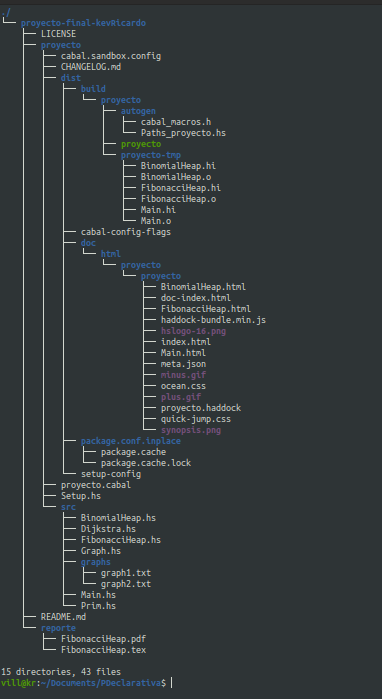
\includegraphics[scale=.5]{img/treepath.png}
\end{center}
Donde podemos encontrar la documentación, el ejecutable, así como el reporte de investigación
\end{document}